\documentclass[journal,10pt,twocolumn]{article}
\usepackage{graphicx}
\usepackage[margin=0.5in]{geometry}
\usepackage[cmex10]{amsmath}
\usepackage{array}
\usepackage{booktabs}
\usepackage{mathtools}
\title{\textbf{Optimization Assignment - 2}}
\author{SRAVANI VUNNAVA}
\date{September 2022}



\let\vec\mathbf
\newcommand{\myvec}[1]{\ensuremath{\begin{pmatrix}#1\end{pmatrix}}}
\newcommand{\mydet}[1]{\ensuremath{\begin{vmatrix}#1\end{vmatrix}}}
\providecommand{\brak}[1]{\ensuremath{\left(#1\right)}}
\providecommand{\lbrak}[1]{\ensuremath{\left(#1\right.}}
\providecommand{\rbrak}[1]{\ensuremath{\left.#1\right)}}
\providecommand{\sbrak}[1]{\ensuremath{{}\left[#1\right]}}

\begin{document}

\maketitle
\paragraph{\textit{Problem Statement} - Show that the surface area of a closed cuboid with square base and a given volume is minimum when it is a cube }
\section*{\large Solution}
\subsection{\textbf{Considerations}}


\begin{tabular}{|c|c|c|}
 \hline
 \textbf{Symbol}&\textbf{Value}&\textbf{Description}\\
 \hline
 l&x&length of cuboid\\
 \hline
 b&x&breadth of cuboid\\
 \hline
	h&$y=\frac{V}{x^2}$&height of cuboid\\
\hline
V&8&Volume of cuboid\\
\hline
\end{tabular}\\
 \begin{equation}
        S = 2x^2+4xy
    \end{equation}
    \begin{equation}
        S = 2x^2 + \frac{4V}{x}
    \end{equation}
    \textbf{minima using conventional method}
    \begin{equation}
        \frac{dS}{dx} = 4x - \frac{4V}{x^2}
    \end{equation}
To find minima
    \begin{equation}
	    \frac{dS}{dx} = 0
	    \end{equation}

	    \begin{equation}
4x - \frac{4V}{x^2} = 0
	    \end{equation}
    \begin{equation}
        V = x^3
    \end{equation}
    \begin{equation}
        x^2y = x^3
    \end{equation}
    \begin{equation}
        y = \frac{x^3}{x^2}
    \end{equation}
    \begin{equation}
        y = x
    \end{equation}
    Hence the height of the cuboid should be equal to the length of square base
\subsection*{\normalsize Gradient descent}
Using gradient descent method we can find its minima ,
    \begin{align}
        x_{n+1} &= x_n - \alpha \nabla f(x_n) \\
        \implies x_{n+1} &= x_n - \alpha \brak{4x_n - \frac{32}{x_n^2}}
    \end{align}
   
Taking $x_0=0.1,\alpha=0.001$ and precision = 0.00000001, values obtained using python are:
    
    \begin{align}
        \boxed{\text{Minima} = 24.00}\\
        \boxed{\text{Minima Point} = 2.00}
    \end{align}
\begin{figure}[t]
 \centering
 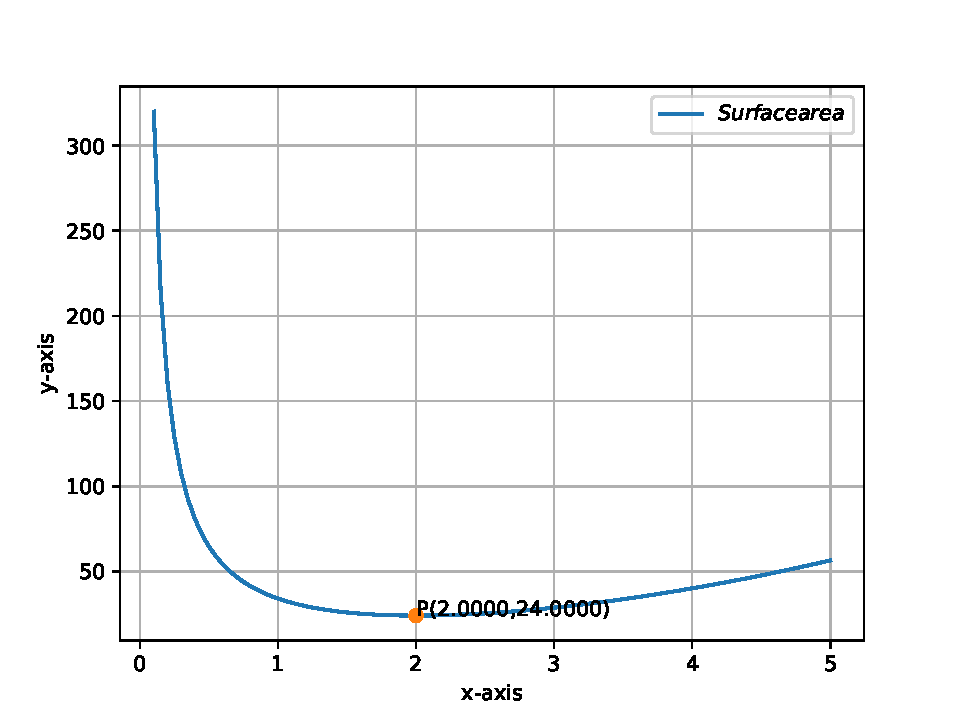
\includegraphics[width=1\columnwidth]{opt.pdf}
 \caption{Graph of Surface area}
 \label{fig:graph_fx}
\end{figure}

\end{document}
